\documentclass[journal, a4paper]{IEEEtran}
\usepackage[T1]{fontenc}       % Encodage le plus étendu
\usepackage[utf8]{inputenc}    % Source Unicode en UTF-8

\usepackage[cyr]{aeguill}
\usepackage[francais]{babel} % Pour la redaction du document en francais


% some very useful LaTeX packages include:

%\usepackage{cite}      % Written by Donald Arseneau
                        % V1.6 and later of IEEEtran pre-defines the format
                        % of the cite.sty package \cite{} output to follow
                        % that of IEEE. Loading the cite package will
                        % result in citation numbers being automatically
                        % sorted and properly "ranged". i.e.,
                        % [1], [9], [2], [7], [5], [6]
                        % (without using cite.sty)
                        % will become:
                        % [1], [2], [5]--[7], [9] (using cite.sty)
                        % cite.sty's \cite will automatically add leading
                        % space, if needed. Use cite.sty's noadjust option
                        % (cite.sty V3.8 and later) if you want to turn this
                        % off. cite.sty is already installed on most LaTeX
                        % systems. The latest version can be obtained at:
                        % http://www.ctan.org/tex-archive/macros/latex/contrib/supported/cite/

\usepackage{graphicx}   % Written by David Carlisle and Sebastian Rahtz
                        % Required if you want graphics, photos, etc.
                        % graphicx.sty is already installed on most LaTeX
                        % systems. The latest version and documentation can
                        % be obtained at:
                        % http://www.ctan.org/tex-archive/macros/latex/required/graphics/
                        % Another good source of documentation is "Using
                        % Imported Graphics in LaTeX2e" by Keith Reckdahl
                        % which can be found as esplatex.ps and epslatex.pdf
                        % at: http://www.ctan.org/tex-archive/info/

%\usepackage{psfrag}    % Written by Craig Barratt, Michael C. Grant,
                        % and David Carlisle
                        % This package allows you to substitute LaTeX
                        % commands for text in imported EPS graphic files.
                        % In this way, LaTeX symbols can be placed into
                        % graphics that have been generated by other
                        % applications. You must use latex->dvips->ps2pdf
                        % workflow (not direct pdf output from pdflatex) if
                        % you wish to use this capability because it works
                        % via some PostScript tricks. Alternatively, the
                        % graphics could be processed as separate files via
                        % psfrag and dvips, then converted to PDF for
                        % inclusion in the main file which uses pdflatex.
                        % Docs are in "The PSfrag System" by Michael C. Grant
                        % and David Carlisle. There is also some information
                        % about using psfrag in "Using Imported Graphics in
                        % LaTeX2e" by Keith Reckdahl which documents the
                        % graphicx package (see above). The psfrag package
                        % and documentation can be obtained at:
                        % http://www.ctan.org/tex-archive/macros/latex/contrib/supported/psfrag/

%\usepackage{subfigure} % Written by Steven Douglas Cochran
                        % This package makes it easy to put subfigures
                        % in your figures. i.e., "figure 1a and 1b"
                        % Docs are in "Using Imported Graphics in LaTeX2e"
                        % by Keith Reckdahl which also documents the graphicx
                        % package (see above). subfigure.sty is already
                        % installed on most LaTeX systems. The latest version
                        % and documentation can be obtained at:
                        % http://www.ctan.org/tex-archive/macros/latex/contrib/supported/subfigure/

\usepackage{url}        % Written by Donald Arseneau
                        % Provides better support for handling and breaking
                        % URLs. url.sty is already installed on most LaTeX
                        % systems. The latest version can be obtained at:
                        % http://www.ctan.org/tex-archive/macros/latex/contrib/other/misc/
                        % Read the url.sty source comments for usage information.

%\usepackage{stfloats}  % Written by Sigitas Tolusis
                        % Gives LaTeX2e the ability to do double column
                        % floats at the bottom of the page as well as the top.
                        % (e.g., "\begin{figure*}[!b]" is not normally
                        % possible in LaTeX2e). This is an invasive package
                        % which rewrites many portions of the LaTeX2e output
                        % routines. It may not work with other packages that
                        % modify the LaTeX2e output routine and/or with other
                        % versions of LaTeX. The latest version and
                        % documentation can be obtained at:
                        % http://www.ctan.org/tex-archive/macros/latex/contrib/supported/sttools/
                        % Documentation is contained in the stfloats.sty
                        % comments as well as in the presfull.pdf file.
                        % Do not use the stfloats baselinefloat ability as
                        % IEEE does not allow \baselineskip to stretch.
                        % Authors submitting work to the IEEE should note
                        % that IEEE rarely uses double column equations and
                        % that authors should try to avoid such use.
                        % Do not be tempted to use the cuted.sty or
                        % midfloat.sty package (by the same author) as IEEE
                        % does not format its papers in such ways.

\usepackage{amsmath}    % From the American Mathematical Society
                        % A popular package that provides many helpful commands
                        % for dealing with mathematics. Note that the AMSmath
                        % package sets \interdisplaylinepenalty to 10000 thus
                        % preventing page breaks from occurring within multiline
                        % equations. Use:
%\interdisplaylinepenalty=2500
                        % after loading amsmath to restore such page breaks
                        % as IEEEtran.cls normally does. amsmath.sty is already
                        % installed on most LaTeX systems. The latest version
                        % and documentation can be obtained at:
                        % http://www.ctan.org/tex-archive/macros/latex/required/amslatex/math/

\usepackage{lipsum} % Dummy text

\usepackage{hyperref} % Hyperlinks

\usepackage{moreverb} % verbatim with indentations


% Other popular packages for formatting tables and equations include:

%\usepackage{array}
% Frank Mittelbach's and David Carlisle's array.sty which improves the
% LaTeX2e array and tabular environments to provide better appearances and
% additional user controls. array.sty is already installed on most systems.
% The latest version and documentation can be obtained at:
% http://www.ctan.org/tex-archive/macros/latex/required/tools/

% V1.6 of IEEEtran contains the IEEEeqnarray family of commands that can
% be used to generate multiline equations as well as matrices, tables, etc.

% Also of notable interest:
% Scott Pakin's eqparbox package for creating (automatically sized) equal
% width boxes. Available:
% http://www.ctan.org/tex-archive/macros/latex/contrib/supported/eqparbox/

% *** Do not adjust lengths that control margins, column widths, etc. ***
% *** Do not use packages that alter fonts (such as pslatex).         ***
% There should be no need to do such things with IEEEtran.cls V1.6 and later.


% En-tête et pied de page
%\usepackage{lastpage}
%\usepackage{fancyhdr}
%\pagestyle{fancy}
%\renewcommand{\sectionmark}[1]{\markright{#1}}
%\fancyhead{}
%%\fancyhead[RO,LE]{\slshape\footnotesize\nouppercase{\rightmark}}
%\fancyhead[LO,RE]{\thetitle}
%\fancyfoot{}
%%\fancyfoot[LO,RE]{\footnotesize\texttt{\thefilename}\\ \textit{\now}}
%%\fancyfoot[C]{-~\thepage~/~\pageref{LastPage}~-}
%\fancyfoot[RO,LE]{\raisebox{-2mm}{\includegraphics{structure/barrette-original}}}
%%
%\fancypagestyle{plain}{ %  Première page ----------------------
%  \fancyhead{}
%  \renewcommand{\headrulewidth}{0pt}
%  \fancyheadoffset[R]{15mm}
%  \fancyhead[L]{
%    \raisebox{-7mm}{
%      \parbox{\textwidth}{
%        \includegraphics{structure/barrette-original} \\ \\
%        \fontsize{8pt}{10pt}\selectfont
%        \sffamily\color{Pantone287}
%        FACULTÉ DES SCIENCES       \\
%        DÉPARTEMENT D'INFORMATIQUE   
%      }
%    }
%  }
%  \fancyhead[R]{
%    \raisebox{-10mm}[0pt][0pt]{\includegraphics[width=120mm]{structure/ULB-ligne-gauche}}
%  }
%  \fancyfoot{}
%  %\fancyfoot[L]{\raisebox{0mm}{}\color{Pantone287}\footnotesize\texttt{\thefilename}\\ \textit{\now}}
%  %\fancyfoot[C]{-~\thepage~/~\pageref{LastPage}~-}
%  \fancyfoot[R]{
%    \raisebox{-12pt}{\includegraphics[height=\footskip]{structure/sceau-mini-b-quadri}}
%  }
%} % Fin de première page
% ---------------------------------------------------------------------------
\usepackage{minted}
\usepackage{algorithm}
\usepackage{algpseudocode}

\usepackage{listings}
% Your document starts here!
\begin{document}

% Define document title and author
	\title{Rapport de projet INFO-F308}
	\author{
		Hugo \textsc{Callens},
		Rayan \textsc{Contuliano Bravo},
		Ziyad \textsc{Haltout Rhouni},
		Manu  \textsc{Mathey-Prevot},
		Moussa \textsc{Tallih}
		\thanks{Superviseur: Valérie \textsc{Gilchrist}}
	}
	\markboth{INFO-F308}{}
	\maketitle


% Write abstract here
\begin{abstract}
	Supposons que vous êtes étudiant à l'Université, et que vous avez besoin de
	trouver votre salle de classe dans un bâtiment que vous ne connaissez pas.
	Comment faire pour la trouver rapidement et sans vous perdre ? L'objectif de
	ce projet est d'utiliser la théorie des graphes afin de trouver le plus court
	chemin entre votre position actuelle et votre salle de classe en utilisant
	les algorithmes de recherche de plus court chemin. Plus besoin de jouer au
	détective pour trouver votre salle de classe grâce à l'application de la
	théorie de graphes.

\end{abstract}

% Each section begins with a \section{title} command
% \section{Introduction}
% 	% \PARstart{}{} creates a tall first letter for this first paragraph
% 	\PARstart{C}{ette} section donne une introduction générale du problème scientifique abordé et décrit la structure de l'article. Des questions souvent abordées ici sont :
% 	\begin{itemize}
% 	\item Quelles sont les applications du problème abordées ?
% 	\item Pourquoi la résolution du problème est importante ?
% 	\end{itemize}	  
\section{Introduction}
	\PARstart{L}{e} problème du plus court chemin dans un graphe est un problème fondamental en informatique et en mathématiques appliquées. Il trouve des applications dans divers domaines tels que la planification des réseaux de transport, la conception de circuits électroniques, la modélisation des réseaux sociaux, etc. La résolution efficace de ce problème est cruciale dans de nombreux contextes pratiques, car elle permet de trouver le chemin le plus court entre deux points dans un réseau, ce qui peut conduire à une optimisation des ressources, une réduction des coûts ou une meilleure planification des trajets. Ainsi, l'étude et le développement d'algorithmes efficaces pour résoudre le problème du plus court chemin revêtent une grande importance tant sur le plan théorique que pratique.

% \section{Etat de l'art}
% 	Cette section permet de décrire l'état de l'art concernant la question abordée (c-à-d les meilleures solutions disponibles à présent) et de positionner votre travail par rapport à cet état de l'art.
% 	Les différents articles que vous avez lus et utilisés doivent être correctement référencés (Exemple: \cite{small},\cite{big}).
% 	Les informations bibliographiques doivent être encodées dans le fichier \texttt{References.bib} avec la syntaxe indiquée par les exemples.
% 	Articles publiés sur une revue scientifique / dans les conference proceedings, ainsi que des livres, sont des exemples de bonnes références.
% 	Par contre, la citation de sources web doit être limitée le plus possible (permis dans le cas de la documentation d'outils informatiques).

\section{État de l'art}
	Cette section vise à présenter un aperçu de l'état actuel des solutions proposées pour le problème du plus court chemin dans un graphe. Les travaux antérieurs dans ce domaine ont produit diverses approches et algorithmes visant à résoudre ce problème de manière efficace. Parmi les méthodes les plus couramment utilisées, on trouve l'algorithme de Dijkstra \cite{dijkstra1959note}, l'algorithme de Bellman-Ford \cite{bellman1958routing}, l'algorithme de Floyd-Warshall \cite{floyd1962algorithm}, et les algorithmes basés sur les tas binaires tels que l'algorithme A* \cite{hart1968formal}. Ces algorithmes ont été largement étudiés et utilisés dans de nombreuses applications pratiques en raison de leur efficacité et de leur polyvalence. \\
\\
	Notamment, l'algorithme de Dijkstra est largement utilisé pour résoudre le problème du plus court chemin dans les graphes pondérés non négatifs, tandis que l'algorithme de Bellman-Ford est plus adapté aux graphes avec des poids négatifs. L'algorithme de Floyd-Warshall, quant à lui, est efficace pour calculer les plus courts chemins entre toutes les paires de sommets dans un graphe, même avec des poids négatifs. Enfin, l'algorithme A* combine la recherche heuristique avec la recherche de coût minimal, ce qui en fait une méthode efficace pour trouver des chemins optimaux dans des graphes de grande taille. \\
\\
	Cependant, malgré les avancées réalisées dans ce domaine, des défis persistent, notamment dans le cas de graphes massifs ou dynamiques. De plus, l'amélioration continue des algorithmes existants et le développement de nouvelles approches restent des sujets de recherche actifs dans la résolution du problème du plus court chemin dans les graphes.

% Main Part
\section{Méthodologie}\label{sec:met}
% 	Cette section doit décrire, en manière détaillée:
% 	\begin{itemize}
% 	\item Les hypothèses de base de votre approche
% 	\item Les fondements mathématiques
% 	\item La méthode proposée
% 	\item Les jeux de données utilisés (si nécessaire)
% 	\item Les instructions nécessaires pour pouvoir reproduire les expériences (par exemple pseudo-code), 
% 	\end{itemize}
	
% 	Ici vous pouvez trouver deux exemples de notation mathématique:
% 	\begin{equation} 
% 	 f(x)=(x+a)(x+b)
% 	\end{equation}

% 	Maxwell's equations:
% \begin{align}
%         B'&=-\nabla \times E,\\
%         E'&=\nabla \times B - 4\pi j,
% \end{align}
\subsection{Création des graphes}
Un graphe est une structure mathématique et informatique composée d'un ensemble de points, appelés nœuds ou sommets, et d'un ensemble de lignes, appelées arêtes ou arcs, reliant ces points. Cette représentation permet d'agencer et de visualiser efficacement des données complexes.

\begin{figure}[h]
	\center
	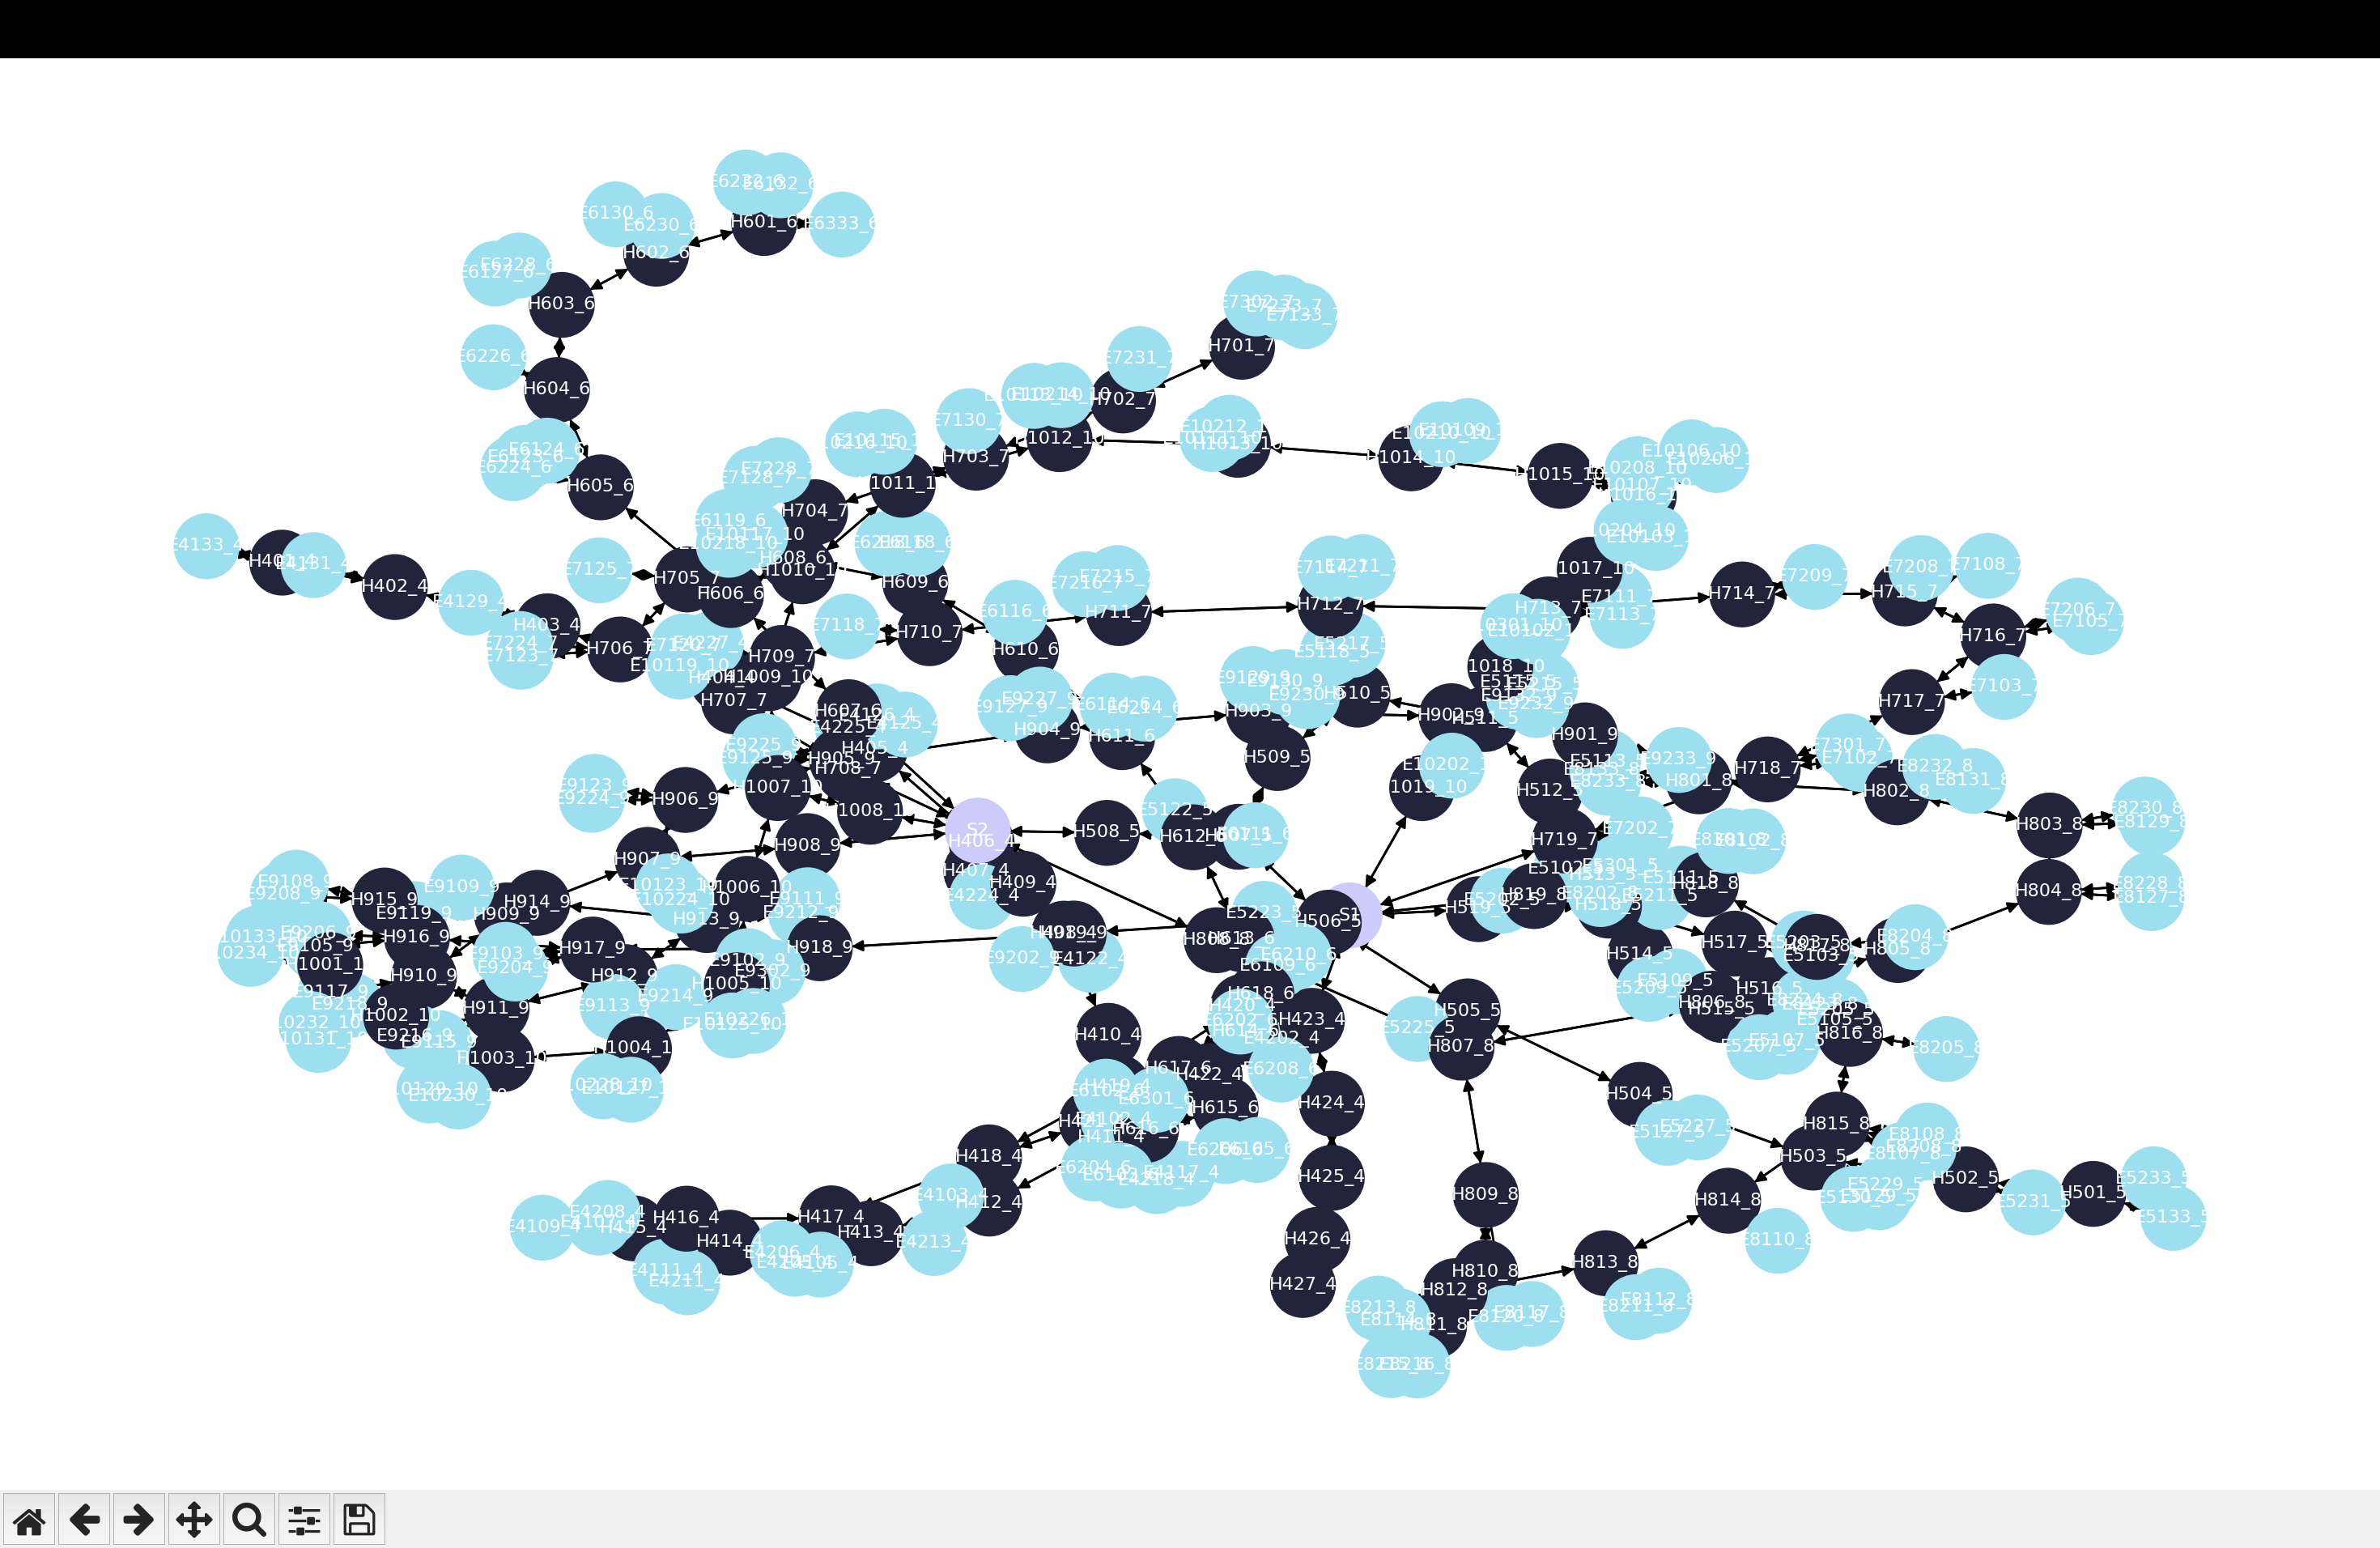
\includegraphics[width=\columnwidth]{img/graph.png}
	\caption{Exemple de graphe}\label{fig:graph}
\end{figure}


La présence d'une arête entre deux nœuds d'un graphe indique l'existence d'une relation ou d'un lien entre ces nœuds. Cette relation peut être de nature diverse, telle qu'une route, une connexion internet, une relation entre deux personnes, etc., et dépend du contexte dans lequel le graphe est utilisé.

Il est possible d'associer un poids à chaque arête d'un graphe. Ce poids est généralement une valeur numérique qui représente de manière abstraite la force, la distance, le coût ou la durée de la relation entre les nœuds reliés par l'arête. Par exemple, dans un graphe représentant une infrastructure réseau, le poids sur les arêtes peut représenter le temps de latence entre deux routeurs. Dans un graphe représentant une carte routière, le poids sur les arêtes peut représenter la distance à parcourir entre deux points.

Trouver le chemin le plus court entre deux nœuds d'un graphe est un problème fondamental en théorie des graphes. Dans ce contexte, le chemin le plus court est défini comme étant le chemin qui a le plus petit poids total. Le poids total d'un chemin est calculé comme la somme des poids de toutes les arêtes du chemin, comme indiqué dans l'équation suivante :

\begin{equation}
\text{Poids total} = \sum_{i \in n} \text{Poids de l'arête i}
\label{eq}
\end{equation}

où $n$ est l'ensemble des arêtes du chemin entre deux nœuds.

Dans ce projet, la théorie des graphes est utilisée pour trouver le plus court chemin entre deux points d'intérêt dans un campus universitaire. Les nœuds du graphe représentent des points clés à l'intérieur ou à l'extérieur des bâtiments, et les arêtes représentent les chemins qui les relient, leur modélisation sera détaillée dans la section suivante. Les poids sur les arêtes quant à eux représente la distance à parcourir entre ces points clés.
\vspace{0.5cm}

\subsubsection{Modélisation d'un bâtiment}
Dans le contexte de ce projet, un ensemble de données composé de plans en vue aérienne de l'ensemble des bâtiments situés sur le campus du Solbosch de l'Université Libre de Bruxelles a été utilisé.

Pour modéliser un bâtiment, chaque pièce a été représentée par un nœud du graphe. Les arêtes du graphe correspondent aux portes et chemins reliant les pièces entre elles. En raison de la qualité insuffisante de l'ensemble de données, l'échelle du plan n'était pas bien définie ou même inexistante. Par conséquent, il a été décidé de considérer que la distance entre chaque pièce était égale à 1. Ainsi, un chemin entre deux pièces correspond simplement au nombre de nœuds à traverser pour passer de l'une à l'autre.

Cependant, cette modélisation présente une limite : la distance réelle entre deux pièces n'est pas prise en compte. Toutefois, cette modélisation simplifiée est suffisante pour les besoins du projet, car il suffit de placer des nœuds à des distances approximativement égales (voir Figure \ref{fig:inside_building}).

\begin{figure}[!hbt]
        \center
	\includegraphics[width=\columnwidth]{img/inside_building}
	\caption{Exemple de modélisation d'un bâtiment en graphe}\label{fig:inside_building}
\end{figure}

Afin de modéliser le graphe d'un bâtiment le plus clairement possible, nous avons décidé d'associer 
un \textit{type} à chaque nœud. Les types possibles sont les suivants : 
\begin{itemize}
	\item \textit{Class}: une salle de classe, auditoire, etc. Généralement l'endroit recherché par les étudiants.
	\item \textit{Hallway}: un couloir, il permet de se déplacer d'un nœud à un autre.
	\item \textit{Stairs}: un escalier, permet de monter ou descendre d'un étage.
	\item \textit{Elevator}: un ascenseur, permet de monter ou descendre d'un étage. Similaire à un escalier 
		sauf que certaines personnes sont obligées de l'utiliser.
	\item \textit{Entrance}: une entrée/sortie d'un bâtiment.
	\item \textit{Unknown}: un nœud dont le type est inconnu.
\end{itemize}

Ils nous permettent de donner des spécificités à des nœuds, comme par exemple le fait que les escaliers et ascenseurs sont à tous les étages, qu'il puisse y avoir plusieurs entrées pour un auditoire, etc \dots
\vspace{0.25cm}

\paragraph{Modélisation en \textbf{JSON}}

Maintenant que la logique de modélisation des bâtiments est claire, nous pouvons réellement le modéliser en 
utilisant la syntaxe \textbf{JSON} suivante : 

\begin{listing}
    \begin{minted}[frame=single,
               framesep=3mm,
               linenos=true,
               xleftmargin=21pt,
               tabsize=4]{js}
{
    "N°étage": [
    	{
    		"id": "",
    		"name": "",
    		"neighbors": [
    			{
    				"id": "",
    				"direction": {
    					"id_pred": ""
    				}
    			}
    		]

    	},
    ]
}
    \end{minted}
    \caption{JSON d'un Bâtiment} 
    \label{lst:json-building}
\end{listing}

Chaque étage aura une liste de nœuds, ces nœuds auront tous comme attributs :  
\begin{itemize}
	\item \textit{id}: un identifiant unique pour chaque nœud. Exemple: \texttt{E123}
	\item \textit{name}: le nom de la salle ou du couloir. Exemple: \texttt{Auditoire Janson}
	\item \textit{neighbors}: une liste de voisins directs du nœud identifiés par leurs nœuds.
\end{itemize}


Cette liste de voisins permet de déterminer les chemins possibles, ainsi que la direction à prendre à partir d'un nœud donné. 
\begin{itemize}
	\item \textit{id}: l'identifiant du voisin. Exemple : \texttt{E124}
	\item \textit{direction}: est un objet qui va contenir chaque prédécesseur possible du nœud dans l'\textbf{id\_pred} et la direction à prendre 
		à partir de celui-ci jusqu'au voisin en passant par le nœud actuel.
\end{itemize}

La direction est très importante. Étant donné qu'il est difficile d'obtenir la position 
de l'utilisateur dans le bâtiment à un étage $e$ et de le diriger en conséquence, nous optons pour cette méthode qui est plus simple à mettre en œuvre.

\vspace{0.5cm}

\subsubsection{Modélisation du campus}
Pour la modélisation d'un campus universitaire, une sélection judicieuse de points est effectuée, correspondant aux nœuds 
d'un graphe. Ces points peuvent représenter des bâtiments, des points d'intérêt, des intersections, etc. Les arêtes du 
graphe représentent les chemins reliant ces points. Les poids sur les arêtes correspondent à la distance en mètres entre 
ces points.

Pour construire le graphe du campus, des points ont été placés sur une carte du campus à l'aide de l'outil en ligne 
Map Marker \cite{mapmarker}. Une fois tous les points placés, les données de latitude et de longitude 
ont été extraites et les voisins directs de chaque point ont été déterminés. Ces informations ont ensuite été traitées 
pour construire le graphe du campus.
\begin{figure}[h]
	\center
	\includegraphics[width=0.6\columnwidth]{img/model_solbosch.png}
	\caption{Exemple de modélisation d'un campus sur le site Map Marker avec les entrées des bâtiments en rouge et les autres en vert}
\end{figure}

% Le graphe du campus est encodé au format JSON sous la forme d'un tableau de nœuds. Chaque nœud est représenté par un objet
% contenant un identifiant, sa latitude et sa longitude, ainsi qu'un tableau de voisins. Chaque voisin est représenté par un 
% objet contenant son identifiant et le poids de l'arête entre le nœud et son voisin. Voici un fichier \texttt{JSON} 
% représentant le graphe du campus:
\vspace{0.25cm}

\paragraph{Modélisation en \textbf{JSON}}
\begin{listing}
    \begin{minted}[frame=single,
               framesep=3mm,
               linenos=true,
               xleftmargin=21pt,
               tabsize=4]{js}
{
    "Campus": [
    	{
    		"id": "",
    		"latitude": "",
            "longitude": "",
    		"neighbors": [
    			{
    				"id": "",
    				"weight": "",
    			}
    		]

    	},
    ]
}
    \end{minted}
    \caption{JSON du campus} 
    \label{lst:json-campus}
\end{listing}
Similairement à la modélisation d'un bâtiment, un campus aura une liste de nœuds, 
ces nœuds auront tous comme attributs 

\begin{itemize}
	\item \textit{id}: un identifiant unique pour chaque nœud. Exemple : \texttt{c9} si nœud ordinaire et \texttt{eJ\_1} si c'est l'entrée d'un bâiment.
        \item \textit{latitude}: Coordonnée de latitude du nœud sur la terre,
        \item \textit{longitude}: Coordonnée de longitude du nœud sur la terre,
	\item \textit{neighbors}: une liste de voisins directs du nœud identifiés par leur nœuds.
\end{itemize}

Cette liste de voisins nous permet de déterminer quels nœuds sont accessibles par d'autres ainsi que la distance entre ceux-ci.

Pour calculer les poids entre les nœuds, un script a été utilisé, faisant appel à la bibliothèque geopy \cite{geopy}
% \href{https://geopy.readthedocs.io/en/stable/#module-geopy.distance}{\texttt{geopy}} 
pour calculer la distance en mètres entre 
deux points géographiques.

\vspace{0.5cm}

\subsubsection{Recherche du plus court chemin}

Dorénavant, il est possible de créer ces graphes en utilisant les fichiers 
\textbf{JSON} ainsi que la librairie NetworkX \cite{networkx}. Des algorithmes de recherche de plus court chemin peuvent maintenant être utilisés pour trouver le chemin le plus court entre deux points de ces graphes.

Pour ce faire, l'algorithme de Dijkstra a été implémenté. Cet algorithme 
utilise le concept de \textit{file à priorité} afin de s'exécuter efficacement.

De manière simplifiée, l'algorithme de Dijkstra fonctionne de la manière suivante : 
Étant donné une \textbf{pile} de nœuds non visités du graphe où la priorité de chaque nœud est initialisé à $+\infty$.
Un nœud de départ est sélectionné et sa priorité est fixée à 0 dans la pile. Tous les voisins de ce nœud sont ensuite visités, car il possède la priorité la plus basse $0 \le + \infty$,
et pour chacun d'eux, leur priorité dans la pile est mise à jour en fonction de la distance entre le nœud actuel et le voisin \textbf{si et seulement si} la priorité du nœud est plus grande que celle qui vient d'être calculée. 
Une fois tous les voisins visités, le nœud actuel (de départ) est retiré de la pile.
Le prochain nœud est sélectionné en prenant celui qui a la priorité la plus basse. Le processus est répété en visitant tous les voisins de ce nœud et en mettant à jour leurs priorités. Ce processus est répété jusqu'à ce que tous les nœuds du graphe aient été visités ou que le nœud d'arrivée ait été atteint.

\begin{algorithm}
\caption{Algorithme de Dijkstra}
\begin{algorithmic}[1]
\State pile $\gets$ graphe.noeuds 
\ForAll{noeud $n$ dans graphe}
    \State n.distance $\gets + \infty$ 
\EndFor
\State départ $\gets$ pile[0]
\State départ.distance $\gets 0$

\While{pile n'est pas vide }
    \State courrant $\gets$ noeud avec la plus petite priorité dans la pile
    \State retire courrant de la pile
    \If{courrant = destination}
        \State \Return chemin trouvé
    \EndIf
    \ForAll{voisin $v$ de courrant}
        \State nouvelle\_distance $\gets$ courrant.distance $+$ distance de courrant à $v$
        \If{nouvelle\_distance < v.distance}
            \State v.distance $\gets$ nouvelle\_distance
        \EndIf
    \EndFor
    
\EndWhile


\end{algorithmic}
\end{algorithm}

\subsubsection{Implémentation d'une application}
Afin d'appliquer le raisonnement des sections précédentes, une application web a été créée afin de faciliter l'utilisation du projet par n'importe qui.

% Un graphe décrivant un campus universitaire a été obtenu et la capacité à rechercher un chemin entre deux nœuds spécifiques a été établie. Le développement d'une interface interactive a été choisi pour faciliter la visualisation et la résolution du problème : permettre à un étudiant de se déplacer efficacement dans son université. Ce processus sera divisé en deux phases distinctes.

% Après avoir obtenu un graphe décrivant un campus universitaire et établi notre capacité à rechercher un chemin entre deux nœuds spécifiques, nous avons opté pour le développement d'une interface interactive. Cette interface vise à faciliter la visualisation et la résolution du problème posé : permettre à un étudiant de se déplacer efficacement dans son université. Ce processus sera divisé en deux phases distinctes.
\vspace{0.25cm}

\paragraph{Implémentation d'une API}
Étant donné que le code est déjà écrit en Python, le développement d'une application moderne a été entrepris, cette application est conforme aux standards actuels des applications dynamiques. Elle se compose d'une interface de programmation applicative (API) renfermant la logique métier de l'application, conjointement à une application cliente qui communique avec cette API par le biais de requêtes HTTP. L'objectif est d'assurer la gestion des interactions avec l'utilisateur via un affichage optimal et faciliter l'utilisation de notre application par nos utilisateurs. Cette api contient deux points d'entrée qui sont les urls : 
\begin{itemize}
\item \texttt{/api/ask} : Ce point d'entrée requiert en paramètres une position géographique et un lieu spécifique au sein de l'université reconnu par l'application. En retour, il fournit le chemin le plus court entre les deux points, à condition que la position géographique se trouve à l'intérieur du campus universitaire.
\item \texttt{/api/ask\_from\_inside} : Ce point d'entrée requiert deux lieux spécifiques au sein de l'université reconnus par l'application en paramètres. Il fournit en retour le chemin le plus court entre ces deux points.
\end{itemize}

Il convient de noter que tout chemin renvoyé par l'API comprend les nœuds, les instructions détaillées pour la transition d'un nœud à un autre, ainsi que des représentations en images 3D pour illustrer ces instructions.
\vspace{0.25cm}
\paragraph{Implémentation de l'interface web}
Par la suite, la création d'une interface graphique s'est avérée nécessaire. Il a donc été utile de développer une page principale permettant à l'utilisateur de choisir entre utiliser sa localisation, récupérée par son navigateur avec son consentement, ou spécifier directement le lieu de départ ainsi que celui de destination. Pour guider l'utilisateur, les instructions nécessaires sont affichées, accompagnées des images correspondantes, de manière séquentielle. L'utilisateur peut parcourir ces instructions en utilisant deux boutons : "Précédent" et "Suivant", jusqu'à atteindre la destination souhaitée.


% Main Part
\section{Résultats}
	En résultat, nous avons une application entièrement fonctionnelle qui répond parfaitement à la problématique. Nous allons donc dans cette section vous la présenter. 
 \subsection{Expérience utilisateur }
Nous allons exposer les étapes distinctes de notre application par lesquelles l'utilisateur procède pour localiser un local. Initialement, deux choix sont proposés à l'utilisateur : utiliser la fonction de localisation GPS ou spécifier manuellement sa position au sein du campus. 
        \begin{figure}[h]
		% Center the figure.
		\begin{center}
		% Include the eps file, scale it such that it's width equals the column width. You can also put width=8cm for example...
		\includegraphics[width=\columnwidth]{img/homepage.png}
		% Create a subtitle for the figure.
		\caption{Lorsque l'utilisateur arrive sur l'application.}
		% Define the label of the figure. It's good to use 'fig:title', so you know that the label belongs to a figure.
		\label{fig:tf_plot}
		\end{center}
	\end{figure}
 \paragraph{À partir de ma position}

Si l'utilisateur décide de se localiser grâce à la fonction de localisation, l'application affiche le chemin le plus court sur une carte, reliant sa position actuelle au bâtiment où se trouve le lieu recherché, comme illustré dans la figure 5. Une fois arrivé dans le bâtiment demandé, il est guidé à l'intérieur du bâtiment à l'aide d'instructions, comme le montrent les figures 6 et 7.
         \begin{figure}[h]
		% Center the figure.
		\begin{center}
		% Include the eps file, scale it such that it's width equals the column width. You can also put width=8cm for example...
		\includegraphics[width=\columnwidth]{img/image.png}
		% Create a subtitle for the figure.
		\caption{L'affichage d'une instruction.}
		% Define the label of the figure. It's good to use 'fig:title', so you know that the label belongs to a figure.
		\label{fig:tf_plot}
		\end{center}
	\end{figure}
        \begin{figure}[h]
		% Center the figure.
		\begin{center}
		% Include the eps file, scale it such that it's width equals the column width. You can also put width=8cm for example...
		\includegraphics[width=\columnwidth]{img/instruction_example.png}
		% Create a subtitle for the figure.
		\caption{L'affichage d'une instruction.}
		% Define the label of the figure. It's good to use 'fig:title', so you know that the label belongs to a figure.
		\label{fig:tf_plot}
		\end{center}
	\end{figure}
         \begin{figure}[!h]
 		% Center the figure.
		% Include the eps file, scale it such that it's width equals the column width. You can also put width=8cm for example...
		\includegraphics[width=\columnwidth]{img/arrival.png}
		% Create a subtitle for the figure.
		\caption{L'affichage de l'arrivée à l'endroit demandé.}
		% Define the label of the figure. It's good to use 'fig:title', so you know that the label belongs to a figure.
		\label{fig:tf_plot}
	\end{figure}
% This is how you define a table: the [!hbt] means that LaTeX is forced (by the !) to place the table exactly here (by h), or if that doesnt work because of a pagebreak or so, it tries to place the table to the bottom of the page (by b) or the top (by t).
\paragraph{À partir d'une classe}
Si l'utilisateur préfère utiliser la localisation du local le plus proche, l'application le guidera dans le bâtiment jusqu'à la sortie ou jusqu'au lieu demandé s'il se trouve dans le même bâtiment, comme indiqué dans les figures 6 et 7. Lorsque l'utilisateur doit passer d'un bâtiment à un autre, l'application agira de la même manière que dans le cas où l'utilisateur sélectionne "À partir de ma position" dès qu'il quitte le bâtiment initial.
\section{Conclusion}
% Cette section contient un rappel des contributions / de résultats importants de votre article et éventuellement une indication sur les perspectives de recherche future dans le même domaine.
Dans ce projet, la théorie des graphes a été appliquée dans le but de trouver le plus court chemin entre 2 points d'intérêt d'un campus universitaire.
Pour ce faire, nous avons modélisé les graphes représentants le campus lui-même et les bâtiments du campus. Ce projet a permis de montrer une application de la théorie des graphes dans la résolution de problèmes du monde réel.
Cependant, il existe encore des défis à relever, notamment dans le cas de graphes massifs ou dynamiques.



\bibliographystyle{unsrt}
\bibliography{bibliography}

% \newpage
		
% \appendices
% \section{Consignes}
% % Main Part
% \subsection*{Document}
% 	% LaTeX takes complete care of your document layout ...
% 	Le rapport doit être rédigé de préférence en \LaTeX{} en utilisant ce template.
% 	La longueur du rapport ne devra pas, en tout cas, dépasser les 6 pages.
% 	Ce rapport doit être \emph{self-contained}, c-à-d il doit pouvoir être lu et compris sans avoir besoin de se documenter ailleurs.



% Your document ends here!
\end{document}